\documentclass{article}
\usepackage{subfig}
\usepackage{tikz}
\usepackage{amssymb}
\usepackage{amsmath}
\usepackage{amsthm}
\usepackage{color}
\usepackage{float}
\usepackage{hyperref}
\usepackage{array}
\usepackage[style=alphabetic,backend=bibtex]{biblatex}
\addbibresource{refs.bib}

\newcommand{\ZZ}{\mathbb{Z}}
\newcommand{\NN}{\mathbb{N}}
\newcommand{\CC}{\mathbb{C}}
\newcommand{\PP}{\mathbb{P}}
\newcommand{\RR} {\mathbb{R}}
\newcommand{\QQ}{\mathbb{Q}}
\newcommand{\FF}{\mathbb{F}}
\newcommand{\isom}{\cong}
\newcommand{\ceil}[1]{\left\lceil #1 \right\rceil}
\newcommand{\Orb}{\mathrm{Orb}}

\newcommand{\xjy}[1]{{\scriptsize \bf {\color{blue}{(xjy)~#1}}}}

\newtheorem{thm}{Theorem}
\newtheorem{defn}[thm]{Definition}
\newtheorem{claim}[thm]{Claim}

\title{Pollard's Rho Algorithm for Discrete Logarithm Computation}
\author{Franklin Harding}
\date{\today}

\begin{document}

\maketitle

\section{Introduction}

Let $G$ be a finite cyclic group for which $g$ is a generator and $h$ is a random group element. The \textit{discrete logarithm problem} (DLP) is to find the smallest non-negative integer $x$ so that $h = g^x$. The existence of an efficient algorithm for solving the DLP would render Diffie-Hellman (DH) key exchange, ElGamal encryption, and various other cryptosystems insecure. In practice, $G$ is typically $\ZZ_p^*$ or the points of an elliptic curve over a finite field of order $p$ ($p$ prime).

Pollard suggested a method for solving DLPs in $\ZZ_p^*$ \cite{Pollard1978} based on his ``rho'' idea initially exploited for factoring \cite{Pollard1975}. The resulting algorithm takes roughly $O(\sqrt{|G|})$ group operations and has negligible space requirements. When combined with the methods of Pohlig and Hellman \cite{Pohlig78}, the run time is reduced to $O(\sqrt{p})$ where $p$ is the largest prime dividing $|G|$.

Shoup demonstrated that generic discrete log algorithms (that succeed with high probability) must perform at least $\Omega(\sqrt{p})$ group operations where $p$ is the largest prime dividing the order of $G$ \cite{Shoup1997}. In other words, Pollard's rho algorithm is essentially the best we can do. While sub-exponential time algorithms exist for $\ZZ_p^*$, Pollard's rho algorithm is still the weapon of choice for elliptic curve DLPs. However, contemporary implementations differ in many ways from Pollard's original rho algorithm. We will discuss these variations and analyze their performance empirically.

\section{Preliminaries}

We use $\NN_0$ to the denote the set of non-negative integers, i.e. $\NN \bigcup \{0\}$. For fixed $n \in \NN$, we write $\ZZ_n$ for the group of integers modulo $n$ with multiplication modulo $n$, and $\ZZ_n^{\times}$, denotes the group of units of $\ZZ_n$. We will mostly deal with $\ZZ_p$ where $p$ is prime, in which case $\ZZ_p^{\times}=\ZZ_p^*=\ZZ_p \setminus \{0\}$. When we deal with a generic group $G$, we assume that for all $g,h \in G$ we can efficiently compute $gh$, and represent each element as a unique binary string.

\section{Pollard's rho method}

Let $W$ be a finite set and $f: W \to W$ be a mapping. For any $w_0 \in W$, the sequence $w_0, f(w_0), f(f(w_0)), \ldots$ is eventually periodic since $W$ is finite. This idea can be used to solve many computational problems and is referred to as the \textit{rho method}. As a warm up and to introduce some terminology, we will describe Pollard's original rho algorithm for solving the DLP in $\ZZ_p^*$; but first, some motivation.

Let $G$ be a group for which $g$ is a generator and $h$ is an arbitrary element. Recall that the DLP is to find the smallest non-negative integer $x$ so that $h=g^x$. If we have some $a,a',b,b' \in \ZZ$ so that $h^a g^b = h^{a'} g^{b'}$ then we can substitute $h=g^x$ yielding $(g^x)^{a-a'} = g^{b'-b}$ which implies $$x(a-a') \equiv b' - b \pmod{|G|},$$
and we can easily compute $x$ so long as $a-a'$ is relatively prime to $|G|$. A naive method for solving DLPs based on this idea is to repeatedly randomly sample $a,b \in \ZZ$ and store $h^a g^b$ in a table until you get a collision. However, the space requirements for this method are too significant for the large groups used in modern cryptography. As you might have guessed, one can combine this idea with Pollard's rho method to produce a more practical algorithm---but first we need to address the elephant in the room: \textit{what if $|G|$ has small factors?}

At first blush this seems like a big issue. If we take $G=\ZZ_p^*$ for some prime $p>2$, then $|G|=p-1$ always has even order, so our toy algorithm fails with high probability. Pollard originally used trial multiplication rather than inversion to solve the linear congruence, which is fairly efficient for most primes. We will use the Pohlig-Hellman algorithm, which allows us to solve a DLP in any group by first solving DLPs in its prime power order subgroups, and then reconstructing a solution to the original DLP via the Chinese Remainder Theorem \cite{Pohlig78}. The ``strong primes'' used in modern cryptography are picked so that $p-1$ has no small prime factors, so $a-a'$ is relatively prime to those prime power subgroup orders with high probability.

\subsection{$\ZZ_p^*$ DLPs}

Let $p$ be a prime for which $g$ is a primitive root, and $h$ be a random element of $\ZZ_p^*$. Recall that the DLP is to find the smallest non-negative integer $x$ so that $h=g^x$. Pollard's original method is as follows. Let $f: \ZZ_p^* \to \ZZ_p^*$ be given by
\begin{align*}
	f(y) = \begin{cases}
		hy & \text{ if } 0 < y < \frac{1}{3}p \\
		y^2 & \text{ if } \frac{1}{3}p < y < \frac{2}{3}p \\
		gy & \text{ if } \frac{2}{3}p < y < p
		\end{cases}.
\end{align*}
Define the sequence $(y_k)$ via the rule $y_0 = 1$ and $y_{i+1}=f(y_i)$ for all $i \in \NN_0$. We refer to $f$ as Pollard's original \textit{iterating function}, and $(y_k)$ as a \textit{psuedorandom walk} in $\ZZ_p^*$. Then there are sequences $(a_i)$ and $(b_i)$ so that $y_i=h^{a_i}g^{b_i}$ which satisfy $a_0=b_0=0$ and the recurrence relations:

\noindent\begin{minipage}{.5\linewidth}
\begin{equation*}
	a_{i+1} = \begin{cases}
		a_i + 1 & \text{ if } 0 < y < \frac{1}{3}p \\
		2 * a_i & \text{ if } \frac{1}{3}p < y < \frac{2}{3}p \\
		a_i & \text { if } \frac{2}{3}p < y < p
		\end{cases}
\end{equation*}
\end{minipage}
\begin{minipage}{.5\linewidth}
\begin{equation*}
	b_{i+1} = \begin{cases}
		b_i & \text{ if } 0 < y < \frac{1}{3}p \\
		2 * b_i & \text{ if } \frac{1}{3}p < y < \frac{2}{3}p \\
		b_i+1 & \text { if } \frac{2}{3}p < y < p
		\end{cases}
\end{equation*}
\end{minipage}
\vspace{1em}

As $\ZZ_p^*$ is finite (of order $p-1$), the psuedorandom walk $(y_k)$ is eventually periodic. That is, there exist distinct indices $i,j \in \NN_0$ such that $y_i=y_j$. In order to find them, we apply Floyd's \textit{cycle-finding} algorithm.
Then we have $h^{a_i}g^{b_i} = h^{a_j}g^{b_j}$ and since $h=g^x$ we have $(g^x)^{a_i-a_j} = g^{b_j-b_i}$ thus $$x(a_i-a_j) \equiv b_j-b_i \pmod {p-1}.$$

Pollard's original rho algorithm for solving the DLP in $\ZZ_p^*$ can easily be modified to work for other groups and indeed, his iterating function $f$ is not unique. However, the fact that we can find sequences $(a_i)$ and $(b_i)$ as described is important. This motivates the following definitions:

\begin{defn}
	Let $G$ be a finite cyclic group and $g,h,y \in G$. An \textbf{iterating function} on $G$ is a function $f: G \to G$ such that for any $a,b \in \NN_0$ such that $y=h^a g^b$ we can efficiently compute $a', b' \in \NN_0$ such that $f(y)=h^{a'} g^{b'}$.
\end{defn}

\begin{defn}
	Let $G$ be a finite cyclic group and $f$ be an iterating function on $G$. A sequence $(y_k)$ is a \textbf{walk} in $G$ with $F$ if $y_0 \in G$ and $y_{k+1} = f(y_{k})$ for all $k \in \NN_0$.
\end{defn}

Clearly $f$ is an iterating function, and $(y_k)$ is a walk in $\ZZ_p^*$ with $f$. In the next section, we will discuss new walks with new iterating functions as proposed by Teske.

\section{Teske's \textit{r-adding} and \textit{r+q-mixed} walks}

Teske came up with new walks and proved both empirically and analytically that they perform better than Pollard's original walk \cite{Teske01}. The idea is essentially unsurprising: an iterating function with ``more rules'' ends up ``looking more random'' so we find a match in fewer steps. Walks without a squaring rule are called \textit{r-adding}; formally:

\begin{defn}
	Let $G$ be a finite cyclic group, $r \in \NN$, and $m_1, \ldots, m_r \in G$. Furthermore, let $v: G \to \{1, 2, \ldots, r\}$ be a hash function and $f$ be an iterating function on $G$. A walk $(y_k)$ on $G$ with $f$ is called \textbf{$r$-adding} if $f$ is of the form $f(y) = y * m_{v(y)}$ for all $y \in G$.
\end{defn}

Teske also generalized Pollard's original walk as \textit{r+q-mixed walks}, which have both multiplication and squaring steps:

\begin{defn}
	Let $G$ be a finite cyclic group, $r,q \in \NN$, and $m_1, \ldots, m_r \in G$. Furthermore, let $v: G \to \{1, \ldots, r+q\}$ be a hash function and $f$ be an iterating function on $G$. A walk $(y_k)$ on $G$ with $f$ is called \textbf{$r+q$-mixed} if $f$ is of the form:
	\begin{align*}
		f(y) = \begin{cases}
			y * m_{v(y)} & \text{ if } v(y) \in \{1,\ldots,r\} \\
			y^2 & \text{ if } v(y) \in \{r+1, \ldots, r+q\}
		\end{cases}.
	\end{align*}
\end{defn}

So Pollard's original iterating function is a $2+1$-mixed walk. The difference between Teske's walks and Pollard's original walk is significant; she found that a $16$-adding walk yields a speed-up by a factor of at least $1.25$ compared to Pollard's original walk. Also, Teske used Knuth's multiplicative hash function, but wrote ``in practical applications, simpler hash functions that can be evaluated faster are certainly preferable.''

\subsection{Hash functions}

Teske's $r$-adding and $r+q$-mixed walks require the use of a hash function in order to partition the group into roughly equal sized sets. In the case of Pollard's original rho algorithm as a $2+1$-mixed walk, this ``hash function'' is essentially $v: \ZZ_p^* \to \{1,2,3\}$ given by
$$v(y) = \begin{cases}
	1 \text{ if } 0 < y < p/3 \\
	2 \text{ if } 2/3p < y < p \\
	3 \text{ if } 1/3p < y < 2/3p
\end{cases}.$$
There is a subtlety of the manner in which a group $G$ is partitioned and the iterating function $f$ is designed in the case of $r+q$-mixed walks; if $e$ is the identity for $G$, then we would like $v(e) \in \{1,\ldots,r\}$ and $m_{v(e)} \neq e$, otherwise $f(e)=e^2=e$ and the walk becomes constant.

Hash functions suitable for this application should be fast and produce a roughly even distribution, but do not need to be cryptographic. Examples include FNV32 and Murmur3.

\section{Cycle-finding}

Let $W$ be a finite set, and $f: W \to W$ be a mapping. Define the sequence $(w_k)_{k \in \NN_0}$ via the rule $w_0 \in W$ and $w_{i+1} = f(w_i)$. Then $(w_k)$ is eventually periodic, so there exist distinct indices $i,j \in \NN_0$ such that $w_i=w_j$. The task of finding such indices is called \textit{finding a match}. More generally, there exist $\lambda \in \NN$ and $\mu \in \NN_0$ such that $w_0,\ldots,w_{\mu + \lambda - 1}$ are distinct and $w_k = w_{k+\lambda}$ for all integers $k \geq \mu$. $\lambda$ is called the \textit{period} and $\mu$ is called the \textit{preperiod}. The process of finding the preperiod and period is called \textit{cycle-finding}. Finding just one match suffices for our purposes (that is, we don't care about $\lambda$ and $\mu$) but most match-finding algorithms are cycle-finding algorithms and vice versa. In this paper, both refer to finding a match.

One of the most basic cycle-finding algorithms (used in Pollard's original rho algorithm) is known as Floyd's cycle-finding algorithm, and works as described in figure $\ref{fig:floyd}$.
\begin{figure}[H]

	\begin{enumerate}
		\item Define $a := w_0$, $b := w_0$, and $i := 0$
		\item Repeat $i := i+1$, $a := f(w_0)$, $b := f(f(w_0))$ until $a=b$
		\item Return $(i,2i)$
	\end{enumerate}
	\caption{Floyd's cycle-finding algorithm \cite{Brent80}}
	\label{fig:floyd}
\end{figure}
If it does not cost much to evaluate $f$, then this is a fairly space and time efficient algorithm. On the other hand, if evaluating $f$ is expensive, then there are better algorithms such as Brent's \cite{Brent80}. Schnorr and Lenstra furter improved upon Brent's algorithm for a specific application of cycle-finding, and their method was generalized by Teske \cite{Teske98}.

The method of \textit{distinguished points} proposed by van Oorschot and Wiener \cite{vOW99} allows for the paralellization of Pollard's rho algorithm. In this method, each processor chooses a random group element to start its walk. Upon each iteration the processor checks whether the group element meets some efficiently testable property, such as the number of leading zeroes in its binary representation. If the group element satisfies that criteria it is considered a distinguished point, and it along with the initial group element is sent to a central repository shared by all processors (otherwise the walk just continues). If the same group element occurs twice in the central repository, then their walks can be reconstructed to find a collision. Given the parallel speed-up, this method essentially renders conventional cycle-finding obsolete.

\section{Group automorphisms}

Let $G=E(\FF_q)$ where $q=p^n$ for some prime $p$ and $n \in \NN$. The negation map $(x,y) \mapsto (x,-y)$ is an automorphism on $G$ of order $2$, and if an iterating function $f$ on $G$ is defined so that $f(y)=f(-y)$, then it is actually defined on the equivalence classes of $G$ under $\pm$. This reduces the average number of iterations to find a match by a factor of $\sqrt{2}$ \cite{DJB11}. If $p=2$ (e.g. Koblitz curves), then a similar idea is to use the Frobenius map $(x,y) \to (x^2,y^2)$, which results in a speed up by a factor of $\sqrt{2n}$ \cite{Gallant2000}. Either method introduces some issues with ``fruitless cycles'' which require some additional work to avoid \cite{Joppe2010}. These are typically the only easily computed automorphisms of small order for elliptic curves.

\iffalse
As a toy example to illustrate this idea, let $F=\FF_2[x]/(x^4+x+1)$ and take $G=F^* \isom (\FF_2(\alpha))^*$ where $\alpha \in F$ is a root of $x^4+x+1 \in \FF_2[x]$. Let $g=\alpha$ and $h=\alpha^2+\alpha$. We want to find $x \in \{0,1,\ldots,2^4-1\}$ so that $g^x=h$. Let $\psi : G \to G$ be given by $\psi(x)=x^2$ (the Frobenius map). Note that $<\psi> = \{\mathrm{Id}, \psi, \psi^2, \psi^3\}$ is a group under function composition. Let $<\psi>$ act on $G$ by $\sigma \cdot y = \sigma(y)$. Then the orbits are the trivial one and
\begin{align*}
	\Orb(\alpha) &= \{\alpha,\alpha^2,\alpha+1,\alpha^2+1\} \\
	\Orb(\alpha^3) &= \{\alpha^3, \alpha^3+\alpha^2, \alpha^3+\alpha^2+\alpha+1, \alpha^3+\alpha\} \\
	\Orb(\alpha^2+\alpha+1) &= \{\alpha^2+\alpha+1,\alpha^2+\alpha\} \\
	\Orb(\alpha^3+\alpha+1) &= \{\alpha^3+\alpha+1,\alpha^3+1,\alpha^3+\alpha^2+1,\alpha^3+\alpha^2+\alpha\}
\end{align*}
The idea is to design an iterating function on $G$ which actually acts on those equivalence classes. That is, we want $f: G \to G$ so that for any $y \in G$ and $y' \in \Orb(y)$, we have $f(y') \in \Orb(f(y))$.


The idea is to design an interating function on $G$ which actually acts on these equivalence classes. That is, we want $f: G \to G$ such that for any $y \in G$ and $y' \in \Orb(y)$, we have $f(y') \in \Orb(f(y))$. In order to accomplish this, we'll first design a well-defined labeling labelling function which sends members of the same equivalence class to some representative integer.

The obvious one works; $\mathcal{L} : G \to \ZZ_{15}$ given by:
\begin{align*}
	\mathcal{L}(y) = \min_{a+b\alpha+c\alpha^2+d\alpha^3 \in \Orb(y)} (2^0a+2^1b+2^2c+2^3d),
\end{align*}
and then we can easily define our iterating function $f: G \to G$ given by $f(y) = y*\psi^{\mathcal{L}(y)}(m_{\mathcal{L}(y)})$ (we skip hashing for simplicity) where e.g.
\begin{align*}
	m_{\mathcal{L}(1)}=g, \qquad
	m_{\mathcal{L}(\alpha)} =h, \qquad
	m_{\mathcal{L}(\alpha^3)}=gh^2, \\
	m_{\mathcal{L}(\alpha^2+\alpha+1)}=g^2h, \qquad
	m_{\mathcal{L}(\alpha^3+\alpha+1)}=g^2h^2.
\end{align*}
Starting with $1$, the walk looks like:
\begin{figure}[H]
	\centering
	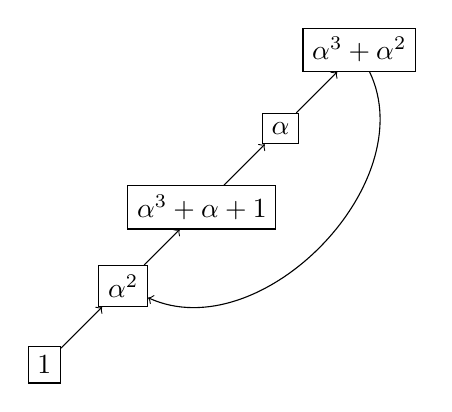
\begin{tikzpicture}
	    \node[shape=rectangle,draw=black] (A) at (0,0) {$1$};
	    \node[shape=rectangle,draw=black] (B) at (1,1) {$\alpha^2$};
	    \node[shape=rectangle,draw=black] (C) at (2,2) {$\alpha^3+\alpha+1$};
	    \node[shape=rectangle,draw=black] (D) at (3,3) {$\alpha$};
	    \node[shape=rectangle,draw=black] (E) at (4,4) {$\alpha^3+\alpha^2$};

	    \path [->] (A) edge (B);
	    \path [->] (B) edge (C);
	    \path [->] (C) edge (D);
	    \path [->] (D) edge (E);
	    \path [->] (E) edge[bend left=70] (B);
	\end{tikzpicture}
	\caption{Walk in the equivalence classes of $(\FF_2[x]/(x^4+x+1))^*$ under the Frobenius automorphism}
\end{figure}
This yields the congruence $(0-14)x=(7-2) \pmod {15}$ and we solve for $x=5$. Indeed, $\alpha^5 = \alpha^2+\alpha$.
\fi

\section{Experiments}

We implemented a number of variations on Pollard's rho algorithm in C using the GNU Multiple Precision (\href{https://gmplib.org/}{https://gmplib.org/}) and Permuted Congruential Generator (\href{https://www.pcg-random.org/}{https://www.pcg-random.org/}) libraries for arbitrary-precision math and random number generation respectively. We tested each variation against prime-order subgroups of $\ZZ_p^*$ and groups of points of an elliptic curve over prime-order finite fields (denoted $E(\FF_p)$). For each type of group, we work with group orders between $10^{n-1}$ and $10^n$ for $3 \leq n \leq 13$. 

Teske showed that if the iterating function on a finite group $G$ behaves like a random mapping and her cycle-finding algorithm based on Schnorr and Lenstra's is used, then we expect a match in approximately $1.416\sqrt{|G|}$ iterations. Thus, she used the metric $$L := \frac{\text{\# of iterations until a cycle is found}}{\sqrt{|G|}}$$ to evaluate the performance of her walk functions experimentally. We will do the same.

\subsection{Walk method}

We compared Pollard's original walk method to a Teske 20-adding walk with Floyd's cycle-finding algorithm and FNV32 hashing.

\begin{figure}[H]
\centering
\subfloat[Teske $20$-adding, FNV32, Floyd]{\begin{tabular}{|b{0.12\textwidth}|c|c|}
	\hline
	digits of subgroup order & average L & DLPs \\
	\hline
	3 & 3.105 & 10000 \\ \hline
	4 & 3.121 & 10000 \\ \hline
	5 & 3.158 & 10000 \\ \hline
	6 & 3.167 & 10000 \\ \hline
	7 & 3.149 & 10000 \\ \hline
	8 & 3.176 & 10000 \\ \hline
	9 & 3.191 & 10000 \\ \hline
	10 & 3.179 & 10000 \\ \hline
	11 & 3.176 & 10000 \\ \hline
	12 & 3.187 & 10000 \\ \hline
	13 & 3.159 & 10000 \\ \hline
\end{tabular}} \quad
\subfloat[Pollard]{\begin{tabular}{|b{0.12\textwidth}|c|c|}
	\hline
	digits of subgroup order & average L & DLPs \\ \hline
	3 & 4.138 & 10000 \\ \hline
	4 & 4.031 & 10000 \\ \hline
	5 & 4.043 & 10000 \\ \hline
	6 & 4.003 & 10000 \\ \hline
	7 & 3.990 & 10000 \\ \hline
	8 & 3.980 & 10000 \\ \hline
	9 & 4.023 & 10000 \\ \hline
	10 & 4.022 & 10000 \\ \hline
	11 & 4.017 & 10000 \\ \hline
	12 & 4.008 & 10000 \\ \hline
	13 & 4.073 & 10000 \\ \hline
\end{tabular}}
\caption{Solving DLPs in prime-order subgroups of $\ZZ_p^*$}
\end{figure}

\iffalse
\begin{defn}
	Let $G$ be a finite cyclic group and $g,h,y \in G$. An \textbf{iterating function} on $G$ is a function $F: G \to G$ such that for any $\alpha,\beta \in \NN_0$ such that $y=g^\alpha h^\beta$ we can efficiently compute $\alpha', \beta' \in \NN_0$ such that $F(y)=g^{\alpha'} h^{\beta'}$.
\end{defn}


\begin{defn}
	Let $G$ be a finite cyclic group, $n \in \NN$, and $M_0, M_1, \ldots, M_{n-1}$ be elements of $G$. Furthermore, let $P$ be a hash function from $G$ to $\ZZ_n$ and $F$ be an iterating function on $G$. A walk $(Y_k)$ with $F$ is called \textbf{$r$-adding} if $F$ is of the form $F(Y) = Y * M_{P(Y)}$ for all $Y \in G$.
\end{defn}
\fi

\section{Conclusion}

Pollard's rho algorithm is known to be one of the fastest and most practical algorithms for computing discrete logarithms, however contemporary implementations take advantage of numerous lesser-known optimizations. Teske came up with new methods of taking random walks in the group called $r$-adding and $r+q$-mixed walks. We implemented Pollard's rho algorithm in C and compared a $20$-adding walk with FNV32 hashing and Floyd's cycle-finding algorithm to Pollard's original rho algorithm with cycle-finding, and showed that Teske's method is significantly faster. Future work would be to study the use of the negation map, other cycle-finding algorithms and hash functions, and the method of distinguished points.

\printbibliography

\end{document}

